\documentclass{beamer}
\usetheme{afm}

\title{Machine Learning}
\author{Matteo Sani - \href{mailto:matteo.sani@unisi.it}{matteo.sani@unisi.it}}

\begin{document}
\begin{frame}[plain]
	\maketitle
\end{frame}

\begin{frame}{Non Linear Models}
  \begin{itemize}
    \item When the target variable $y$ has a more complicated relationship with the independent variables $X$ and linear models are not working any more we need to move to \emph{non-linear models}.
    \item If the model is not known it is possible to use \emph{machine learning techniques} in order to infer its characteristics directly from the dataset.
    \item Machine Learning (ML) is a subset of artificial intelligence (AI) that deals with creating models that learn or improve performance based on the data they use. Artificial intelligence is a generic term and refers to systems or machines that imitate human intelligence.
  \end{itemize}
\end{frame}

\begin{frame}{Neural Networks}
  \begin{itemize}
  \item Artificial Neural Networks (ANN or simply NN) are information processing models that are developed by inspiring from the working principles of human brain.
  \item \emph{Their most essential property is the ability of learning from sample sets.}
  \item The basic unit of ANN architecture are \emph{neurons}. 
    \begin{figure}[htb]
      \begin{center}
        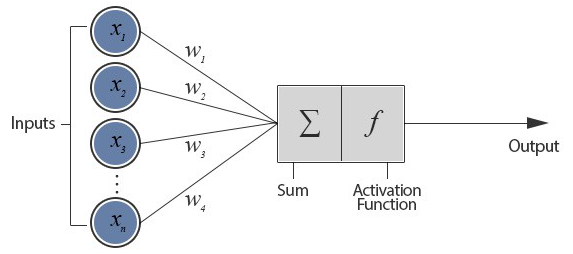
\includegraphics[width=0.55\linewidth]{neuron}
      \end{center}
    \end{figure}
    \begin{equation}  
      \textrm{Inputs} = \sum_{i=1}^{N} x_i w_i +w_0 = \Sigma \rightarrow = f(\Sigma) \rightarrow \textrm{Output}
    \end{equation}
  \end{itemize}
\end{frame}

\begin{frame}{Activation Function}
  \begin{itemize}
  \item The \emph{activation function} is used to add non-linearity to the respons of the neuron.
    \begin{columns}
      \column{0.6\linewidth}
    \item There are many different types of activation function
      \begin{itemize}
      \item \emph{step function} which returns just 0 or 1 according to the input value;
      \item \emph{sigmoid} which can be thought of as the continuous version of the step function);
      \item \emph{rectified Linear Unit} (ReLU); 
      \item \emph{hyperbolic tangent} (tanh).
      \end{itemize}
      \column{0.4\linewidth}      
      \begin{figure}[htb]
        \begin{center}
          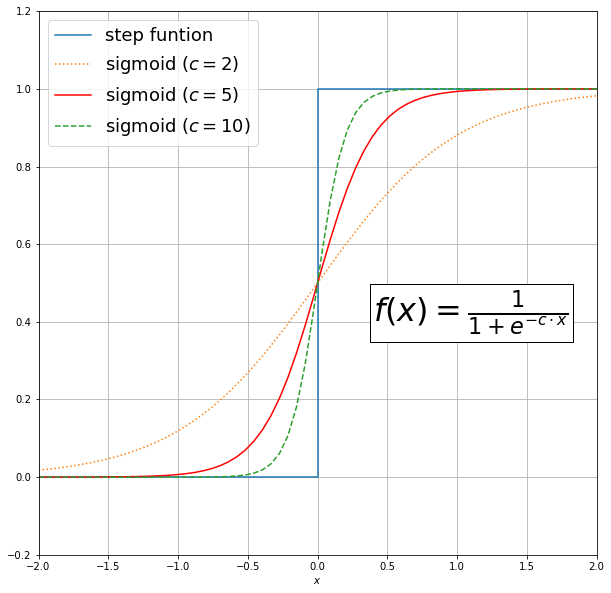
\includegraphics[width=0.90\linewidth]{sigmoid}
        \end{center}
      \end{figure}
    \end{columns}
  \end{itemize}
\end{frame}

\begin{frame}{Supervised Training of a Neuron}
  In the process of training a neuron we would like to teach it to give the "correct" output providing a certain input (hence the name \emph{supervised}).
  \begin{enumerate}
    \item Inputs from the \emph{training} set are presented to the neuron one after the other together with the target output;
    \item the neuron weights are modified in order to make the neuron output as close as possible to the target;
    \item when an entire pass through all of the input training vectors is completed (an \emph{epoch}) the neuron has learnt;
  \end{enumerate}
  Actually we can present many times the same set to the neuron to make it learn better (but not too many times, see \emph{overfitting}).
\end{frame}

\begin{frame}{Multilayered Neural Networks}
  \begin{itemize}
    \item Using just a neuron is a too simple architecture. The next step is to put together more neurons in \emph{layers}.
      \begin{figure}[htb]
        \begin{center}
          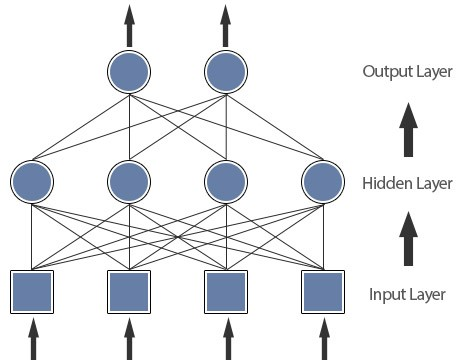
\includegraphics[width=0.40\linewidth]{multilayer}
        \end{center}
      \end{figure}
    \item In a multilayered NN each neuron from the \emph{input layer} is fed up to each neuron in the next hidden layer, and from there to each neuron on the output layer. 
    \item There can be any number of neurons per layer.
  \end{itemize}
\end{frame}

\begin{frame}{Neural Network Design}
  \begin{itemize}
    \item There is no rule to guide developers into the design of a neural network in terms of number of layers and neuron per layer. 
    \item The most common strategy is \emph{trial and error} where you pick up the solution giving the best accuracy. 
    \item In general a larger number of nodes is better to catch highly structured data with a lot of feature although it may require larger training sample to work correctly.
    \item \textbf{As a rule of thumb a NN with just one hidden layer with a number of neurons averaging the inputs and outputs is sufficient in most cases.}
  \end{itemize}
\end{frame}

\begin{frame}{Training a Multilayered Neural Network}
  The training of a multilayered NN follows similar these steps:
  \begin{enumerate}
    \item present a training sample to the neural network and compute the network output obtained by calculating activations of each neuron of each layer;
    \item calculate the \emph{loss} as the difference between the NN predicted and the target output;
    \item "re-adjust" the weights of the network such that the difference with the target output decreases;
    \item continue the process for each input several times (epochs).
  \end{enumerate}
\end{frame}

\begin{frame}{Training a Multilayered Neural Network}
  \begin{figure}[htb]
    \begin{center}
      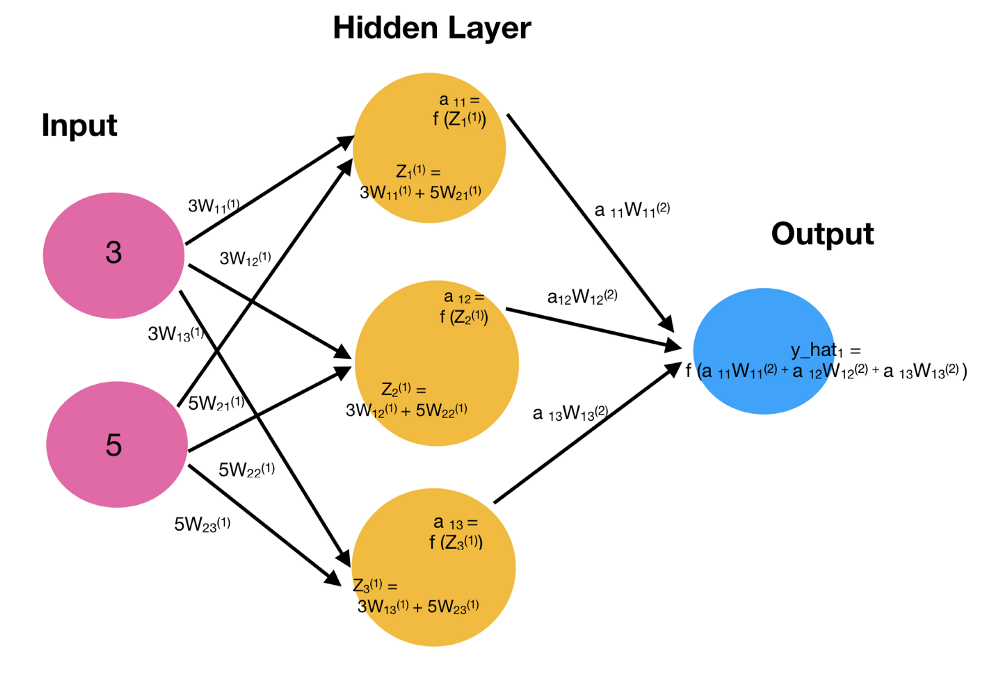
\includegraphics[width=0.65\linewidth]{training_nn}
    \end{center}
  \end{figure}
\end{frame}

\begin{frame}{Loss Function}
  \begin{itemize}
  \item The NN loss is computed by the \emph{loss function}, possible choices are
    \begin{itemize}
      \item Mean Absolute Error (MAE): the average of the absolute value of the differences between the predictions and true values. It represents how far off we are on average from the correct value;
      \item Root Mean Squared Error (MSE): the square root of the average of the squared differences between the predictions and true values. It penalizes larger errors more heavily and is commonly used in regression tasks.
    \end{itemize}
  \end{itemize}
\end{frame}

\begin{frame}{Back Propagation}
  \emph{Back propagation} is the algorithm used to reduce the loss function: the current loss is "propagated" backwards to previous layers, where it is used to modify the weights.
  \begin{columns}
    \column{0.5\linewidth}
    \begin{figure}[htb]
      \begin{center}
        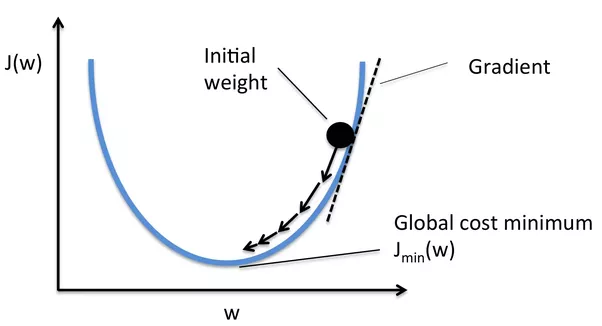
\includegraphics[width=0.85\linewidth]{loss_function}
      \end{center}
    \end{figure}
    \column{0.5\linewidth}
    \begin{equation}
      \min_{w} L(w_{11}, w_{12},\ldots) \implies \frac{\partial L}{\partial w_{ij}} = 0
    \end{equation}
  \end{columns}  
  Weights are modified using a function called \emph{optimization function} (we will use \emph{Adam} (Adaptive Moment Estimation) as optimizator in the following but there are more).
\end{frame}

\begin{frame}{Classification}
  \begin{itemize}
  \item  Is the process of finding a function to split the dataset into classes based on different parameters. 
  \item The goal is to find the mapping function between the input and the \emph{discrete} output($y$).
    \item Email spam detection: the model is trained on the basis of millions of emails on different parameters, and whenever it receives a new email, it identifies whether the email is spam or not.
    \item Classification algorithms can also be in speech recognition, car plates identification, etc.
  \end{itemize}
\end{frame}

\begin{frame}{Regression}
  \begin{itemize}
  \item It is the process of finding the correlations between dependent and independent variables. 
    \item The goal is to find the mapping function to map the input variable to the \emph{continuous} output variable.
    \item Housing price prediction: the input data can be different home features and the output prediction will be pricing estimate. 
    \item In general whenever we are dealing with function approximation this kind of algorithms can be applied.
  \end{itemize}
\end{frame}

\begin{frame}{Overfitting (Overtraining)}
  \begin{itemize}
  \item Increasing too much the number of epochs may lead to overfitting: the NN learns too well the training sample but its performance degrade substantially in an independent sample.
  \item It is required to split the available sample in two parts: training and testing (e.g. 80\% and 20\%) 
  \item \emph{training} to perform the setting of the weights;
  \item \emph{testing} to cross-check the performance in an independent sample. 
  \item To check if this is the case we can \emph{evaluate} our NN with both the training ad the testing samples. 
  \item If the losses are comparable the NN is ok otherwise if the training losses are much smaller than the testing we had overfitting.
  \item In this second case if we need more accuracy we need to either increase the training sample or to change the NN design.
  \end{itemize}
\end{frame}

\begin{frame}{A Feature Not a Bug}
  \begin{itemize}
    \item If you ran the previous example you would most likely obtain different results.
    \item \textbf{This is not a bug but a feature of NN}, let's see which are the possible sources for such discrepancies.
    \item \emph{Stochastic learning algorithm}: NN algorithm is stochastic i.e. its behaviour incorporates elements of randomness (beware that stochastic does not mean learning a random model). 
    \item Their randomness comes from:
      \begin{itemize}
        \item the \emph{random initial weights}, which allow the model to try learning from a different starting point in the search space each time; 
        \item the \emph{random shuffle of examples during training}, which ensures that each gradient estimate and weight update is slightly different.
      \end{itemize}
  \end{itemize}
\end{frame}

\begin{frame}{A Feature Not a Bug}
  \begin{itemize}
    \item The impact is that each time it is run on the same data, it learns a slightly different model and when evaluated, may have a slightly different performance.
    \item You can control randomness by setting the seed used by the pseudorandom number generator: although this is not a good approach in practice:
      \begin{itemize}
      \item \textbf{there is no best seed for any algorithm}; 
      \item you need to summarize the performance by fitting multiple times a model on your dataset and averaging its predictions.
      \end{itemize}
  \end{itemize}
\end{frame}
\end{document}

